\documentclass[a4paper,12pt]{article} %размер бумаги устанавливаем А4, шрифт 12пунктов
% \usepackage[T2A]{fontenc}
\usepackage[utf8]{inputenc}%кодировка
\usepackage[english,russian]{babel}%используем русский и английский языки с переносами
% \usepackage{amssymb,amsfonts,amsmath,cite,enumerate,float,indentfirst} %пакеты расширений
\usepackage[pdftex]{graphicx} %вставка графики
\graphicspath{{images/}}%путь к рисункам
\usepackage{minted}
\usepackage{listings}
\usepackage{subcaption}

\usepackage{algorithmicx}
\usepackage{algpseudocode}
% \floatname{algorithm}{Procedure}

% \usepackage{algorithm2e}
%  % Перевод плагина
\SetKwInput{KwData}{Исходные параметры}
\SetKwInput{KwResult}{Результат}
\SetKwInput{KwIn}{Входные данные}
\SetKwInput{KwOut}{Выходные данные}
\SetKwIF{If}{ElseIf}{Else}{Если}{тогда}{иначе\ если}{иначе}{конец\ условия}
\SetKwFor{While}{До\ тех\ пор,\ пока}{выполнять}{конец\ цикла}
\SetKw{KwTo}{от}
\SetKw{KwRet}{возвратить}
\SetKw{Return}{Возвратить}
\SetKwBlock{Begin}{Начало\ блока}{конец\ блока}
\SetKwSwitch{Switch}{Case}{Other}{Проверить\ значение}{и\ выполнить}{вариант}{в\ противном\ случае}{конец\ варианта}{конец\ проверки\ значений}
\SetKwFor{For}{Цикл}{выполнять}{Конец\ цикла}
\SetKwFor{ForEach}{Для\ каждого}{выполнять}{Конец\ цикла}
\SetKwRepeat{Repeat}{Повторять}{До\ тех\ пор,\ пока}
\SetAlgorithmName{Алгоритм}{алгоритм}{Список алгоритмов}


% \makeatletter
% \renewcommand{\@biblabel}[1]{#1.} % Заменяем библиографию с квадратных скобок на точку:
% \makeatother

\usepackage{geometry} % Меняем поля страницы
\geometry{left=2.5cm}% левое поле
\geometry{right=1.5cm}% правое поле
\geometry{top=2cm}% верхнее поле
\geometry{bottom=2cm}% нижнее поле

% \usepackage{hyperref}
% \hypersetup{%
%     pdfborder = {0 0 0}
% }
\usepackage[hidelinks]{hyperref}

\usepackage{wrapfig}

% \renewcommand{\theenumi}{\arabic{enumi}}% Меняем везде перечисления на цифра.цифра
% \renewcommand{\labelenumi}{\arabic{enumi}}% Меняем везде перечисления на цифра.цифра
% \renewcommand{\theenumii}{.\arabic{enumii}}% Меняем везде перечисления на цифра.цифра
% \renewcommand{\labelenumii}{\arabic{enumi}.\arabic{enumii}.}% Меняем везде перечисления на цифра.цифра
% \renewcommand{\theenumiii}{.\arabic{enumiii}}% Меняем везде перечисления на цифра.цифра
% \renewcommand{\labelenumiii}{\arabic{enumi}.\arabic{enumii}.\arabic{enumiii}.}% Меняем везде перечисления на цифра.цифра

% \newcommand{\imgh}[3]{\begin{figure}[h]\center{\includegraphics[width=#1]{#2}}\caption{#3}\label{ris:#2}\end{figure}}

\lstdefinelanguage{llang}{
	keywords={skip, do, while, read, write, if, then, else},
	sensitive=true,
	%%basicstyle=\small,
	commentstyle=\scriptsize\rmfamily,
	keywordstyle=\ttfamily\underbar,
	identifierstyle=\ttfamily,
	basewidth={0.5em,0.5em},
	columns=fixed,
	fontadjust=true,
	literate={->}{{$\to$}}1
}

\lstset{
	language=llang
}

\begin{document}
\begin{titlepage}
\newpage

\begin{center}
	\textbf{
		Санкт-Петербургский Государственный Университет \\
		Математико-механический факультет \\
	}
	Кафедра системного программирования
\end{center}

\vspace{15em}

\begin{center}
\Large Форматирование текста программ на основе комбинаторов, сопоставления с образцом и синтаксических шаблонов \\ 
\end{center}

\vspace{2em}

\begin{center}
Курсовая работа студента 445 группы \\
Подкопаева Антона Викторовича

\end{center}

\vspace{10em}

Научный руководитель\dotfill
к.ф.-м.н. Д. Ю. Булычев

% \hfill доц. каф. систем. прогр.

\vspace{\fill}

\begin{center}
Санкт-Петербург \\2013
\end{center}

\end{titlepage}

\newpage
\tableofcontents % это оглавление, которое генерируется автоматически
\newpage
\section*{Введение}

Ручное управление памятью в языках, подобных C++, является источником большого количества трудно отслеживаемых ошибок, наличия которых можно было бы
избежать, сделав процесс управления памятью автоматическим. \textit{Сборка мусора} является одним из способов автоматического управления памятью, при
котором освобождение памяти выводится из-под контроля ПО на прикладном уровне. При автоматическом управлении программист не может явно влиять на распределение
объектов в памяти, у него есть лишь
косвенные способы сделать это с помощью использования тех или иных языковых конструкций. В идеальном случае, для рационального использования
памяти необходимо освобождать память, занимаемую объектами, которые более не будут использованы программой. Поскольку точно определить, что
объект не будет использован в дальнейшем, невозможно, на практике используют критерий доступности. \textit{Доступность} --- это консервативное
приближение используемости. \textit{Мусором}, в таком случае, называют объект, все пути доступа к которому уже разрушены, а память из-под него
ещё не освобождена. В некоторое, заранее определенное время, например, в простейшем случае, когда перестаёт хватать свободной памяти, выполнение
программы временно приостанавливается и запускается процесс \textit{сборки мусора}, который освобождает всю или ту, что возможно, память,
занятую мусором, после чего управление возвращается обратно программе. \textit{Сборщиком мусора} называется компонент, производящий \textit{сборку мусора}.

Процесс \textit{сборки мусора}, в простейшем случае, делят на три этапа:
\begin{enumerate}
\item \textit{Построение корневого множества}. На этом этапе строится множество объектов, которые считаются изначально доступными.
Такие объекты называются \textit{корнями} (англ. roots). Данное построение
аксиоматично, т.е. основывается на некотором наборе правил, согласно которым те или иные элементы считаются доступными. Данный этап является неотъемлемой
частью любого сборщика мусора.
\item \textit{Маркировка}. Начиная с множества, построенного на предыдущем этапе, происходит сканирование памяти, и все объекты, до которых возможно
добраться из построенного корневого множества, считаются доступными; оставшиеся объекты считаются мусором.
\item \textit{Освобождение}. Происходит сканирование кучи, в течение которого память из-под всех элементов, помеченных как мусор или не отмеченных как
доступные, освобождается.
\end{enumerate}

Есть несколько требований, которые должны быть выполнены для реализации сборки мусора:
\begin{enumerate}
\item Возможность построения корневого множества. Иными словами, необходимо иметь возможность идентифицировать все указатели в программном стеке, регистрах
и статической области памяти.
\item Должна присутствовать возможность определить все указатели из любого объекта на другие элементы кучи.
\end{enumerate}
В таких языках, как LISP или JAVA все условия соблюдаются, и в них успешно используется технология сборки мусора, в то время как, например,
в языке C не все условия выполняются. В языках, где не соблюдаются хотя бы одно из вышеперечисленных условий, возможна исключительна
\textit{консервативная сборка мусора}.
\textit{Консервативной} называется такая сборка мусора, при которой любой элемент данных, значение которого может быть истолковано, как указатель на
некоторый элемент кучи, считается  таковым. Консервативный подход к сборке мусора не позволяет собрать весь мусор, что может стать проблемой при обработке
большого количества данных. Неконсервативная сборка мусора лишена подобного недостатка и способна освободить всю память программы, более не
являющуюся доступной. \textit{Неконсервативным} или  \textit{точным сборком мусора} называется сборщик мусора, имеющий возможность точно распознать
все указатели в памяти. Иными словами, точный сборщик мусора --- это сборщик мусора, не использующий консервативный подход.

В C++ не соблюдаются требования, необходимые для сборки сборки мусора, реализовать точный сборщик мусора без ограничений
на использование некоторых примитивов языка не представляется возможным.
Более того, в C++ имеется ряд технических сложностей, затрудняющих реализацию точного сборщика мусора.
Тем не менее, в случае соблюдения программистом некоторых соглашений на програмный код,
точная сборка мусора становится возможной и в C++.

Целями работы является реализация основных примитивов библиотеки неконсервативной сборки мусора для C++,
обеспечение возможности совмещения ручного и автоматического управления памятью.
\newpage
\section{Некоторые средства автоматизации\\
управления памятью для С++}

Одним из наиболее широко используемых средств автоматизации управления памятью в
контексте языка С++ являются ``умные указатели'' (smart pointers). ``Умный указатель''~---
это специальный объект, который хранит указатель на участок динамически отведенной области
памяти и определяет некоторую дисциплину обращения с этом указателем. Иногда следование
этой дисциплине является лишь соглашением, и тогда ``умный указатель'' является всего лишь
способом идентифицировать необходимость правильного обращения с данными; однако довольно часто
``умные указатели'' действительно определенным образом ограничивают набор возможных
способов манипулирования данными за счет использования декларативных возможностей языка С++.

Простейший ``умный указатель'' может выглядеть так:

\begin{lstlisting}
    template <typename T> class smart_pointer {
      T *m_obj; // Указатель на динамические данные
      public:
        // Конструктор получает исходный указатель 
        smart_pointer (T *obj) : m_obj(obj) {}
        // Деструктор удаляет адресуемые данные
        ~smart_pointer () { delete m_obj; }
        // Перегруженные операторы для обращения к данным
        T* operator-> () { return m_obj; }
        T& operator*  () { return *m_obj; }
    }
\end{lstlisting}

Такой указатель позволяет обеспечить автоматическое освобождение области динамической памяти, если 
время её жизни можно ограничить временем жизни самого ``умного указателя''. При этом никак не
контролируется, что сам ``умный указатель'' используется правильно --- например, что конструктор
получает действительно адрес в куче или что для данного адреса создан только один ``умный указатель''.

Другим примером ``умного указателя''является \lstinline{Boost::scoped_ptr}\footnote{\url{http://www.boost.org/doc/libs/1_39_0/libs/smart_ptr/scoped_ptr.htm}} 
библиотеки BOOST\footnote{\url{http://www.boost.org}}. Его основное отличие от приведенного выше~--- отсутствие возможности копирования и присваивания (а,
значит, и передачи параметром в функцию). Эти ограничения не исключают возможность неправильного использования, но позволяют избежать некоторых из них.

Еще одним вариантом является \lstinline{auto_ptr}\footnote{\url{http://www.cplusplus.com/reference/memory/auto_ptr}}. Этот указатель разрешает
операции копирования и передачи параметром, но при этом ``опустошается'' содержимое источника. Таким образом, указатели не копируются, 
а ``перемещаются'', что позволяет избежать ситуации, когда происходит несколько попыток освободить одну и ту же область памяти из-за хранения 
её адреса разными ``умными указателями''. С другой стороны, теперь не гарантируется, что ``умный указатель'' всегда указывает на правильные данные ---
в какой-то момент он может ``испортиться''. В силу этого такие указатели нельзя использовать в контейнерах STL. Для таких целей используются
\lstinline{std::shared_ptr}.

\lstinline{shared_ptr}\footnote{\url{http://www.cplusplus.com/reference/memory/shared_ptr}}~--- это ``умный указатель'' с подсчетом ссылок. Это значит, 
что с каждой областью памяти, адресуемой \lstinline{shared_ptr}, ассоциирована переменная, которая хранит количество указателей, которые ссылаются на начало
этой области памяти. Если эта переменная становится равной нулю, то область освобождается. Счетчик инкрементируется при каждом вызове оператора копирования 
или оператора присваивания. У \lstinline{shared_ptr} есть оператор приведения к типу \lstinline{bool}, что позволяет проверять, указывает ли он на что-нибудь.
Использование \lstinline{shared_ptr} может обеспечить сравнительно безопасную автоматизацию управления памятью, однако неприятности все же возможны. Во-первых,
наличие указателя \lstinline{shared_ptr} не на начало динамически отведенной области памяти не гарантирует её сохранения; кроме того, циклические
ссылки приводят к образованию неудаляемого мусора; наконец, возможна ситуация лавинообразного освобождения памяти с возникновением непредсказуемой
задержки.

\newpage
\section{Реализация принтера, основанного на шаблонах}

Основной целью данной работы была разработка прототипа принтера, который бы использовал для печати шаблоны.

\subsection{Описание общего подхода}

Работа принтера разбивается на два этапа: подготовка шаблонов и непосредственно печать синтаксического дерева.

На подготовительном этапе из файла с шаблонами языковых конструкций строится набор образцов. \textit{Образцом} назовем пару из текста шаблона и обобщенного синтаксического дерева шаблона. Дерево шаблона --- обобщенное, так как на месте некоторых узлов стоят специальные метки, которые хранят информацию об ограничениях на текстовое представление соответствующих узлов.

Во время основной фазы работы принтера дерево, которое необходимо непачатать, сравнивается с деревьями из образцов. В случае согласованности образца и дерева для печати используется текст образца, в который на места меток вставляются представления соответствующих поддеревьев.

% Благодаря шаблонам, необходимый результат получается просто и наглядно.

\subsection{Шаблон}

Внутри шаблона используется специальный язык разметки. Символы “\lstinline{@-}” на позиции поддерева синтаксической конструкции означают, что для применения данного шаблона поддерево должно быть напечатано в одну строку. Семантика символов “\lstinline{@* N @*}” совпадает с семантикой “\lstinline{@-}” с точностью до того, что напечатанное поддерево должно занимать строку длины не более N. Символы “\lstinline{@| @|}” означают, что соответствующее поддерево может быть напечатано и на нескольких строках. Для выделения отдельных шаблонов используются строки “\lstinline{t_start}”, “\lstinline{t_end}”.

Рассмотрим пример шаблонов для конструкции “\lstinline{write}” языка L (см. рис. \ref{fig:writeTmplt1} и \ref{fig:writeTmplt2}).
Эти шаблоны задают именно такое представление \lstinline{write}”, которого мы добивались в обзоре принтер-библиотек.

\begin{figure}[h!]
	\begin{subfigure}[h]{0.45\textwidth}
		\lstinputlisting{Podkopaev/codes/writeTmplt1.l}
		\caption{}
		\label{fig:writeTmplt1}
	\end{subfigure}
	\begin{subfigure}[h]{0.45\textwidth}
		\lstinputlisting{Podkopaev/codes/writeTmplt2.l}
		\caption{}
		\label{fig:writeTmplt2}
	\end{subfigure}
	\caption{Шаблоны для конструкции “\lstinline{write}”}
\end{figure}

Рассмотрим шаблоны для конструкции “\lstinline{if-then-else}” (см. рис. \ref{fig:flatGoodIfTmplt} и \ref{fig:multBadIfTmplt}).
С помощью них можно напечатать дерево, изображенное на рисунке~\ref{fig:nestedIf} (см. рис. \ref{fig:nestedIfCode}).

\begin{figure}[h!]
	\begin{subfigure}[h]{0.45\textwidth}
		\lstinputlisting{Podkopaev/codes/flatGoodIfTmplt.l}
		\caption{Однострочный вариант}
		\label{fig:flatGoodIfTmplt}
	\end{subfigure}
	
	\begin{subfigure}[h]{0.45\textwidth}
		\lstinputlisting{Podkopaev/codes/multBadIfTmplt.l}
		\caption{Многострочный вариант}
		\label{fig:multBadIfTmplt}
	\end{subfigure}
	\caption{Шаблоны для конструкции “\lstinline{if-then-else}”}
	\label{fig:ifTmplt}
\end{figure}

\begin{figure}[h!]
	\centering
	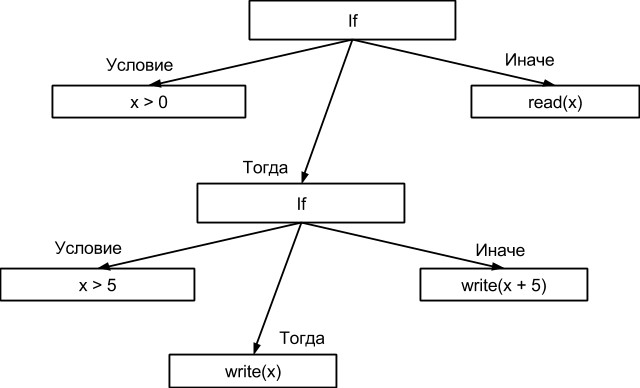
\includegraphics[width=0.6\textwidth]{nestedIf}
	\caption{Пример дерева “\lstinline{if-then-else}”}
	\label{fig:nestedIf}
\end{figure}

\begin{figure}[h!]
	\centering
	\lstinputlisting{Podkopaev/codes/nestedIf.l}
	\caption{Представление с помощью шаблонов с рис. \ref{fig:ifTmplt}}
	\label{fig:nestedIfCode}
\end{figure}

Одним из неочевидных свойств шаблонов является то, что с их помощью можно выражать не только базовые конструкции языка.
Например, можно завести отдельный шаблон для случая, когда обе ветки конструкции “\lstinline{if-then-else}” представляют собой операторы “\lstinline{write}” (см. рис. \ref{fig:writeNestedInIf}). Если добавить такой шаблон, то пример дерева с рисунка~\ref{fig:nestedIf} получит новое представление (см. рис. \ref{fig:nestedIfNew}).

\begin{figure}[h!]
	\lstinputlisting{Podkopaev/codes/writeNestedInIf.t}
	\caption{Пример задания шаблона для сложной конструкции}
	\label{fig:writeNestedInIf}
\end{figure}

\begin{figure}[h!]
	\lstinputlisting{Podkopaev/codes/nestedIfNew.l}
	\caption{Представление дерева с рис. \ref{fig:nestedIf} с использованием шаблона с рис. \ref{fig:writeNestedInIf}}
	\label{fig:nestedIfNew}
\end{figure}

\subsection{Построение образцов}

Для работы принтера неообходимо иметь возможность сравнивать синтаксическое представление шаблонов с деревом, которое печатается. Поэтому необходим синтаксический анализатор, который может разбирать шаблонные конструкции в рамках целевого языка. Удобным способом разработать данный анализатор является использование расширяемого синтаксического анализатора целевого языка. В результате работы расширенного анализатора получается набор образцов. В узлах синтаксического дерева, соответствующих меткам шаблонов, хранится информация о положении метки внутри текста образца, чтобы на этапе печати документа знать, куда вставлять представления поддеревьев.

\newpage

\subsection{Печать дерева с использованием набора образцов}

На этапе, когда уже имеются необходимые образцы, происходит их сопоставление с синтаксическим деревом, переданным на печать.
Псевдокод алгоритма приведен ниже (см. рис. \ref{fig:comparePseudoCode}).

\begin{figure}[h!]
	\begin{algorithmic}
		\State{H --- ассоциативный массив, связывает деревья с их текстовым представлением}
		\State{M --- набор образцов для языковых конструкций}

		\State{ }
		\State{Комментарий: По дереву строит его текстовое представление}
		\Function{print}{$tree$}
			\If{$tree \in H$}
				\State\Return{$H[tree]$}
			\Else
				\State{Вызов print для поддеревьев $tree$}
				\State\Return{\Call{templateIter}{$tree$}}
			\EndIf
		\EndFunction

		\State{ }
		\State{Комментарий: Перебирает все образцы и пытается их применить к дереву}
		\Function{templateIter}{$tree$}
			\ForAll{$(templateTree, text) \in M$}
				\State{Комментарий: В случае исключения, переходит к новому элементу $M$}
				\State{$list$ := \Call{templateCompare}{$tree, templateTree$}}
				\State{$H[tree]$ := построенное представление для $tree$ по $list$ и $text$}
				\State\Return{$H[tree]$}
			\EndFor
		\EndFunction

		\State{ }
		\State{Комментарий: Возвращает список координат метки в тексте шаблона и соответствующее текстовое представление поддерева}
		\Function{templateCompare}{$tree, templateTree$}
			\If{$tree$ и $templateTree$ одного типа}
				\State{Вызвать $templateCompare$ для соответствующих поддеревьев}
				\State\Return{соединенный список результатов вызова для поддеревьев}
			\EndIf

			\If{$templateTree$ является меткой}
				\If{$H[tree]$ соответствует ограничениям метки}
					\State\Return{$[($координаты метки$, H[tree])]$}
				\Else
					\State{создать исключение}
				\EndIf
			\EndIf

			\State{Создать исключение, т.к. переданные деревья разной структуры}
		\EndFunction
		
	\end{algorithmic}
	\caption{Псевдокод сопоставления дерева с набором образцов}
	\label{fig:comparePseudoCode}
\end{figure}

Из псевдокода видно, что в случае, если для какого-нибудь поддерева не найдется соответствующий образец, то дерево невозможно будет напечатать. То есть множество образцов должно быть достаточным. Это естественное ограничение.

% Попробуем оценить время работы алгоритма. Пусть $|M|$ --- количество образцов, $height(T)$ --- высота дерева, а $K$ --- максимальное число поддеревьев у узла синтаксического дерева целевого языка. Тогда время работы алгоритма можно оценить как $O((|M| \times K)^{height(T)} )$.

Попробуем оценить время работы алгоритма. Для каждого узла дерева, переданного принтеру, вычисляется следующее:
\begin{enumerate}
	\item текстовое представление для детей;
	\item сравнение с имеющимися образцами;
	\item текстовое представление узла по выбранному образцу и представлениям детей.
\end{enumerate}

Текстовое представление вычисляется для каждого узла один раз. Сравнение с образцами занимает $O(B \times |M|)$ времени, где $B$ --- максимальное число узлов в дереве образца, а $|M|$ --- количество образцов. Построение текстового представления по выбранному образцу занимает $O(A)$, где $A$ --- максимальное количество меток в шаблоне, но так как очевидно, что $A \leq B$, то оценку можно заменить на $O(B)$. Таким образом, оценка на работу алгоритма для дерева с $T$ узлами равна $O(T \times B \times |M|)$.

Для сравнения, если реализовать аналогичный принтер с помощью библиотеки Азеро и Свиерстры, то это приведет к экспоненциальному от размера дерева расчету текстового представления. В случае библиотек Хьюза и Вадлера похожий принтер будет иметь квадратичную сложность.

\newpage

\subsection{Реализованный принтер}

Описанный подход был реализован на примере принтера языка L, написанного на языке OCaml\footnote{http://ocaml.org}. Для написания синтаксического анализатора была использована библиотека Ostap\footnote{http://oops.math.spbu.ru/projects/ostap}.

В качестве примера работы принтера с разными шаблонами рассмотрим уже упоминавшуюся программу быстрого возведения в степень (см. рис. \ref{fig:lEx}).
С помощью шаблонов, приведенных в дополнении~\ref{app:1}, принтер печатает программу в виде, изображенном на рисунке \ref{fig:firstTemplatePow}.

\begin{figure}[h!]
	\lstinputlisting{Podkopaev/codes/firstTemplatePow.l}
	\caption{Программа быстрого возведения в степень на языке L, напечатанная с помощью шаблонов из дополнения~\ref{app:1}}
	\label{fig:firstTemplatePow}
\end{figure}

Шаблоны, приведенные в дополнении~\ref{app:2}, представляют программу несколько иным образом (см. рис. \ref{fig:secondTemplatePow}).

\begin{figure}[h!]
	\lstinputlisting{Podkopaev/codes/secondTemplatePow.l}
	\caption{Программа быстрого возведения в степень на языке L, напечатанная с помощью шаблонов из дополнения~\ref{app:2}}
	\label{fig:secondTemplatePow}
\end{figure}

Из приведенных примеров виден один из недостатков реализации. Если присмотреться к конструкции \lstinline{if-then-else}, то можно заметить, что \lstinline{then} и \lstinline{else} находятся на разных уровнях. Естественно, это нежелательный результат. Пока эта проблема не решена, в дальнейшем планируется разобраться с этой проблемой путем расширения языка шаблонов.
\newpage
\section*{Заключение}

% \subsection*{Результаты}
% \addcontentsline{toc}{subsection}{Результаты}

В рамках данной работы достигнуты следующие результаты:
\begin{enumerate}
\item Для задачи поиска оптимальной раскладки документа,
определенного с помощью комбинаторов из \cite{swierstra}, на заданную ширину
конструктивно доказана ее линейность относительно размеров дерева комбинаторов;
\item Разработан подход к заданию принтеров с помощью образцов для языков программирования;
\item Реализован плагин форматирования программных текстов на языке Java для IntelliJ IDEA
в рамках апробации общего подхода.
\end{enumerate}


% \subsection*{Дальнейшая работа}
% \addcontentsline{toc}{subsection}{Дальнейшая работа}

Существует несколько направлений для развития данной работы.
В рамках плагина стоит добавить
анализ эталонного репозитория на полноту, чтобы для полученного по
эталонному коду принтера можно было гарантировать возможность
обработки любого абстрактного синтаксического дерева Java.
Также для возможности практического применения необходимо повысить
производительность плагина.
Для общего подхода самой важной задачей является разработка
абстрагированной от целевого языка программной системы. Кроме того,
необходимо получить способ описания порядка поддеревьев для тех
случаев, когда он не задан явно синтаксисом языка.

\newpage
\addcontentsline{toc}{section}{Список литературы}

% \bibliographystyle{plain}
% \bibliography{articles}

\begin{thebibliography}{9001}

\bibitem{myCoursePaper} А.Подкопаев. Форматирование текста программ на основе комбинаторов, сопоставления с образцом и синтаксических шаблонов
// Курсовая работа, кафедра Системного Программирования, МатМех СПбГУ, 2013.

% \bibitem{haskellImpl} Реализация и тестовые примеры
% оптимальных принтер-комбинаторов на Haskell, \cd{http://github.com/anlun/polynomialPPCombinators}

\bibitem{burs} A.V.Aho, M.Ganapathi, S.W.K.Tjiang. Code Generation Using Tree Matching and Dynamic Programming // ACM Transactions on Programming Languages and Systems, 
11(4), 1989.


\bibitem{maintance} G.Alkhatib. The maintenance problem of application software:
an empirical analysis // Journal of Software Maintenance, 4(2):83–104, 1992.

\bibitem{swierstra} P.Azero, S.D.Swierstra. Optimal Pretty-Printing Combinators. \cd{http://www.cs.ruu.nl/groups/ST/Software/PP}, 1998.

\bibitem{swiComb} P.Azero, S.D.Swierstra, J.Saraiava. Designing and Implementing Combinator Languages // Advanced Functional Programming, 1999.

\bibitem{chitil} O.Chitil. Pretty Printing with Lazy Dequeues // ACM Trans. Program. Lang. Syst. 27(1), 2005.

\bibitem{tata} H.Comon, M.Dauchet, R.Gilleron \emph{et al}. Tree Automata Techniques and Applications, \cd{http://www.grappa.univ-lille3.fr/tata}, 2007.

\bibitem{learning} F.Corbo, C.Del Grosso, M.Di Penta. Smart Formatter: Learning Coding Style from
Existing Source Code // Software Maintenance. ICSM 2007. IEEE International Conference, pp.525,526, 2-5, 2007.

\bibitem{poset} C.Daskalakis, R.M.Karp, E.Mossel, S.Riesenfeld, E.Verbin.
Sorting and Selection in Posets.
In Proceedings of the twentieth Annual ACM-SIAM Symposium on Discrete
Algorithms (SODA '09). Society for Industrial and Applied Mathematics, Philadelphia, PA, USA, 392-401, 2009.

\bibitem{hughes} J.Hughes. The Design of a Pretty-printing Library // Advanced Functional Programming, 1995.

\bibitem{eclipse} S.Jackson, P.Devanbu, K.Ma. Stable, Flexible, Peephole Pretty-Printing // Journal Science of Computer Programming, 72(1-2), 2008.

\bibitem{jongeEveryOccasion} M.De Jonge. A Pretty-Printer for Every Occasion // Proceedings of the 2nd International Symposium on Constructing 
Software Engineering Tools, 2000.

\bibitem{jongeReengine} M.De Jonge. Pretty-printing for Software Reengineering // Proceedings of the International Conference On Software Maintenance, 2002.

\bibitem{kiselyov} O.Kiselyov, S.Peyton-Jones, A.Sabry. Lazy vs. Yield: Incremental, Linear Pretty-Printing // 10th Asian Symposium on Programming Languages and Systems, 
2012.

\bibitem{oppen} D.C.Oppen. Pretty-printing // ACM Transactions on Programming Languages and Systems, 2(4), 1980.

\bibitem{peytonJones} Peyton Jones S. Haskell Pretty-printer Library // \cd{http://www.haskell.org/ghc/docs/latest/html/libraries/pretty-1.1.1.0/Text-PrettyPrint.html}, 1997.

\bibitem{podkopaevBoulytchev} A.Podkopaev, D.Boulytchev.
Polynomial-Time Optimal Pretty-Printing Combinators with Choice // Принято на PSI-2014. 

\bibitem{rendelInvert} T.Rendel, K.Ostermann. Invertible syntax descriptions: unifying parsing and pretty printing // SIGPLAN Not. 45, 11, 1-12, 2010.

\bibitem{codingStandarts} J.Shore. The Art of Agile Development. O'Relly Media, 2010.

\bibitem{swierstra04} S.D.Swierstra. Linear, Online, Functional Pretty Printing (corrected and extended version).
Technical report, UU-CS-2004-025a. Institute of Information and Computing Sciences, Utrecht University, 2004.

\bibitem{swierstraChitil} S.D.Swierstra, O. Chitil. Linear, Bounded, Functional Pretty-printing // J. Funct. Program., Vol. 19,
2009.

\bibitem{brandBox} M.Van den Brand, E.Visser. Generation of Formatters for Context-free Languages // ACM Trans. Softw. Eng. Methodol., 5(1), 1996.

\bibitem{wadler} P.Wadler. A Prettier Printer // The Fun of Programming. Palgrave MacMillan, 2003.


\end{thebibliography}

\newpage
%\appendix
\setcounter{subsection}{0}
\renewcommand\thesubsection{\Alph{subsection}}

\section*{Приложения}
\subsection{Первый вариант набора шаблонов для языка L}
\label{app:1}
\lstinputlisting{Podkopaev/codes/l_template.t}

\subsection{Второй вариант набора шаблонов для языка L}
\label{app:2}

\lstinputlisting{Podkopaev/codes/l_template_2.t}

\renewcommand\thesubsection{\arabic{subsection}}

\end{document}
